\section{Description}
The Flyweight Pattern (FWP) is a structural pattern. According to Wikipeia "structural design patterns are design patterns that ease the design by identifying a simple way to realize relationships between entities" (see \url{http://en.wikipedia.org/wiki/Structural_pattern}). FWP upholds this definition by prescribing a way to have a large number of objects share common properties. This is done by providing references to shared data - typically through a Flyweight Factory (Factory Method Pattern). The primary goal of FWP is to optimize memory usage in terms of how much space objects occupy in memory, but there can also be a significant boost to the speed of an application. However, the amount of space and time being saved depends on the specific data structures and in some cases we gain nothing by using FWP. When to use and when not to use FWP will be discussed in the conclusion.\\

When researching the Flyweight pattern some special terminology is often being used. Here an independent-state refers to data that is shared between objects (intrinsic state) and a dependent-state refers to data unique to an object, that cannot be shared (extrinsic state).\\

A common example in articles on the subject is, how to implement character objects in a word processor application. In this example characters share data such as font, colour and size (intrinsic states) with other characters, while a character's position is always unique (extrinsic state). The idea is now to obtain references to the shared data objects through the Flyweight Factory and pass them into the character objects. It is important to notice that space is only saved if the reference pointers are smaller in size than the objects they point to. On the other hand it is usually always faster to pass a reference to an object already created compared to creating a new object, so using the Flyweight Factory can still be a good solution although the amount of memory used is not reduced. The diagram \ref{fig:FlyweightPattern} shows an example of an FWP implementation:

\begin{figure}[h]
	\centering
	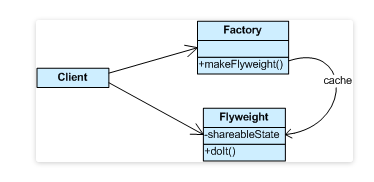
\includegraphics[width=0.7\linewidth]{Content/Pattern_example.png}
	\caption{Simple Flyweight Pattern class diagram (borrowed from http://synvistech.com/blogs/flyweight-design-pattern/).}

	\label{fig:FlyweightPattern}
\end{figure}

 